\documentclass{article}
\usepackage[a4paper]{geometry}
\usepackage{bookmark}
\usepackage{listings}
\usepackage{amsmath,amsfonts,amsthm,amssymb,mathtools}
\usepackage[italian]{babel}
\usepackage{graphicx}
\usepackage{multirow}
\usepackage{wrapfig}
\title{\Huge{Pendolo fisico}}
\author{\huge{Giosué Aiello, Domenico Fenili, Francesco Sermi}}
\date{14 Novembre 2023}
\usepackage{xcolor}

\definecolor{codegreen}{rgb}{0,0.6,0}
\definecolor{codegray}{rgb}{0.5,0.5,0.5}
\definecolor{codepurple}{rgb}{0.58,0,0.82}
\definecolor{backcolour}{rgb}{0.95,0.95,0.92}

\lstdefinestyle{code}{
    backgroundcolor=\color{backcolour},   
    commentstyle=\color{codegreen},
    keywordstyle=\color{magenta},
    numberstyle=\tiny\color{codegray},
    stringstyle=\color{codepurple},
    basicstyle=\ttfamily\footnotesize,
    breakatwhitespace=false,         
    breaklines=true,                 
    captionpos=b,                    
    keepspaces=true,                 
    numbers=left,                    
    numbersep=5pt,                  
    showspaces=false,                
    showstringspaces=false,
    showtabs=false,                  
    tabsize=2
}
\lstset{style=code}
\begin{document}

\maketitle
\pagebreak
\tableofcontents
\pagebreak

\section{Scopo dell'esperienza}
Lo scopo di questa esperienza è quello di misurare il periodo di un pendolo fisico in funzione della distanza del perno di rotazione dal centro di massa.

\section{Cenni teorici}

\begin{figure}[h!]
	\centering
	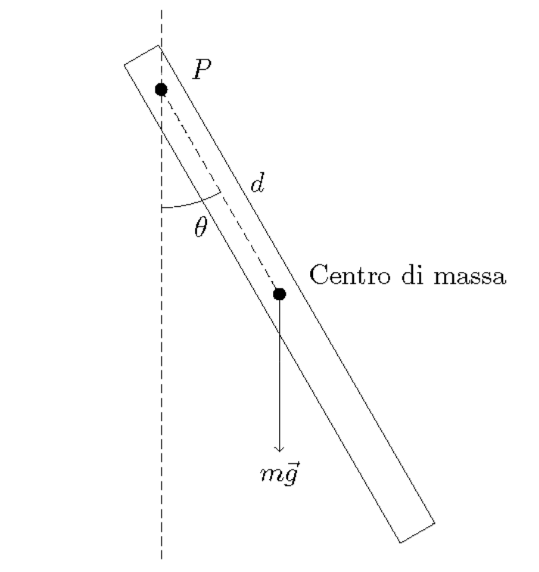
\includegraphics[scale=0.35]{pendolo_fisico.png}
	\caption{Schema del nostro apparato sperimentale}
	\label{fig:schema_pendolo}
\end{figure}
\par\smallskip\noindent Un oggetto fissato ad un punto di sospensione $P$ (che dista $d$ dal centro di massa) e soggetto alla gravità costituisce un pendolo fisico. Se questo corpo viene spostato di un angolo $\theta$ dalla sua posizione di equilibrio, il momento torcente della forza di gravità (rispetto al punto di sospensione $P$) vale:
\begin{equation}
	\tau = -mgd\sin{\theta}
\end{equation}
che, per $\theta << 10^\circ - 15^\circ$ possiamo esprimere $sin(\theta)$ utilizzando la formula di espansione in serie di Taylor al primo ordine:
\begin{equation*}
	\sin{\theta} = \sum_{n = 0}^{+\infty} \frac{(-1)^n}{(2n+1)!}\theta^{2n+1} = \theta + o(\theta^3) \approx \theta
\end{equation*}
Pertanto possiamo riscrivere il momento torcente della forza di gravità come:
\begin{equation*}
	\tau = -mgd\theta
\end{equation*}
E per la seconda equazione cardinale si ha che:
\begin{equation}
	\tau = \frac{dL}{dt}
\end{equation}
e sapendo che il momento angolare di un pendolo fisico risulta essere pari a $L = I\omega$ e $\omega = \frac{d\theta}{dt}$ si ha che:
$$
	\tau = \frac{dL}{dt} = I\frac{d}{dt} \left(\frac{d\theta}{dt} \right) = I\frac{d^2 \theta}{dt^2}
$$
Combinando la $(1)$ e la $(2)$:
\begin{equation}
	I\frac{d^2 \theta}{dt^2} = -mgd\theta \implies \frac{d^2 \theta}{dt^2} + \frac{mgd}{I}\theta = 0 
\end{equation}
Siamo dinanzi ad un'equazione differenziale di secondo ordine a coefficienti costanti omogenea di un moto armonico con pulsazione e periodo di oscillazione dati da:
$$\omega_0 = \sqrt{\frac{mgd}{I}} \, \, \, \, \, \, T_0 = 2\pi\sqrt{\frac{I}{mgd}}$$
Utilizzando il teorema degli assi paralleli, possiamo concludere che il momento di inerzia dell'oggetto fisico risulta essere:
$$
	I = I_{cm} + md^2 = \frac{ml^2}{12} + md^2
$$
Possiamo quindi riscrivere la formula nella seguente maniera:
\begin{equation}
	T(d) = \sqrt{\frac{m(l^2 + d^2)}{mgd}} = \sqrt{\frac{\frac{l^2}{12} + d^2}{gd}}
\end{equation}
\section{Apparato sperimentale e strumenti}

\begin{itemize}
	\item Strumenti 
	\begin{itemize}
		\item Metro a nastro, risoluzione $0.1$ cm;
		\item Calibro ventesimale, risoluzione $0.05$ mm;
		\item Cronometro, risoluzione $0.01 $ s.
	\end{itemize}
	\item Materiali
	\begin{itemize}
		\item Asta metallica forata;
		\item Un supporto di sospensione;
	\end{itemize}
\end{itemize}

\section{Descrizione delle misure}

--Completare

Per fare le misurazioni

\begin{table}[h!]
	\hspace{-0.1\textwidth}	
	\begin{minipage}{0.1\textwidth}
		\centering
		\begin{tabular}{ | r | c | c | }
			\hline
			\multirow{2}{5em}{Numero prova}& $\tau (s)$ & $d (cm) $ \\
			& $\pm 0.01$ & $\pm 0.1$ \\
			\hline
			1 & 16.09 & \multirow{7}{1em}{$95.0$} \\ \cline{1-2}
			2 & 15.90 & \\	\cline{1-2}
			3 & 	15.73 & \\	\cline{1-2}
			4 &	15.93 & \\	\cline{1-2}
			5 &	15.89 & \\	\cline{1-2}
			6 &	15.67 & \\	\cline{1-2}
			7 &	16.00 & \\	\cline{1-2}
			\hline
		\end{tabular}
	\end{minipage}
	\hspace{0.3\textwidth}
	\begin{minipage}{0.1\textwidth}
		\centering
		\begin{tabular}{ | r | c | c | }
    		\hline
    		\multirow{2}{5em}{Numero prova} & $\tau$ (s) & $d$ (cm) \\
    		& $\pm 0.01$ & $\pm 0.1$ \\
    		\hline
    		1 & 15.31 & \multirow{7}{*}{85.0} \\ \cline{1-2}
    		2 & 15.42 & \\ \cline{1-2}
    		3 & 15.30 & \\ \cline{1-2}
    		4 & 15.56 & \\ \cline{1-2}
    		5 & 15.29 & \\ \cline{1-2}
    		6 & 15.50 & \\ \cline{1-2}
    		7 & 15.53 & \\ \cline{1-2}
    		\hline
		\end{tabular}
	\end{minipage}
	\hspace{0.3\textwidth}
	\begin{minipage}{0.1\textwidth}
		\centering
		\begin{tabular}{ | r | c | c | }
    		\hline
    		\multirow{2}{5em}{Numero prova} & $\tau$ (s) & $d$ (cm) \\
    		& $\pm 0.01$ & $\pm 0.1$ \\
    		\hline
    		1 & 15.75 & \multirow{7}{*}{75.0} \\ \cline{1-2}
    		2 & 15.66 & \\ \cline{1-2}
    		3 & 15.73 & \\ \cline{1-2}
    		4 & 15.61 & \\ \cline{1-2}
    		5 & 15.67 & \\ \cline{1-2}
    		6 & 15.80 & \\ \cline{1-2}
    		7 & 15.67 & \\ \cline{1-2}
    		\hline
		\end{tabular}
	\end{minipage}
\end{table}
\begin{table}[h!]
	\hspace{-0.1\textwidth}	
	\begin{minipage}{0.1\textwidth}
			\begin{tabular}{ | r | c | c | }
    				\hline
    				\multirow{2}{5em}{Numero prova} & $\tau$ (s) & $d$ (cm) \\
    				& $\pm 0.01$ & $\pm 0.1$ \\
    				\hline
    				1 & 15.75 & \multirow{7}{*}{75.0} \\ \cline{1-2}
    				2 & 15.66 & \\ \cline{1-2}
    				3 & 15.73 & \\ \cline{1-2}
    				4 & 15.61 & \\ \cline{1-2}
    				5 & 15.67 & \\ \cline{1-2}
    				6 & 15.80 & \\ \cline{1-2}
    				7 & 15.67 & \\ \cline{1-2}
    				\hline
			\end{tabular}
	\end{minipage}
	\hspace{0.3\textwidth}
	\begin{minipage}{0.1\textwidth}
			\begin{tabular}{ | r | c | c | }
    				\hline
    				\multirow{2}{5em}{Numero prova} & $\tau$ (s) & $d$ (cm) \\
    				& $\pm 0.01$ & $\pm 0.1$ \\
    				\hline
    				1 & 15.75 & \multirow{7}{*}{75.0} \\ \cline{1-2}
    				2 & 15.66 & \\ \cline{1-2}
    				3 & 15.73 & \\ \cline{1-2}
    				4 & 15.61 & \\ \cline{1-2}
    				5 & 15.67 & \\ \cline{1-2}
    				6 & 15.80 & \\ \cline{1-2}
    				7 & 15.67 & \\ \cline{1-2}
    				\hline
			\end{tabular}
	\end{minipage}
	\hspace{0.3\textwidth}
	\begin{minipage}{0.1\textwidth}
			\begin{tabular}{ | r | c | c | }
    				\hline
    				\multirow{2}{5em}{Numero prova} & $\tau$ (s) & $d$ (cm) \\
    				& $\pm 0.01$ & $\pm 0.1$ \\
    				\hline
    				1 & 15.75 & \multirow{7}{*}{75.0} \\ \cline{1-2}
    				2 & 15.66 & \\ \cline{1-2}
    				3 & 15.73 & \\ \cline{1-2}
    				4 & 15.61 & \\ \cline{1-2}
    				5 & 15.67 & \\ \cline{1-2}
    				6 & 15.80 & \\ \cline{1-2}
    				7 & 15.67 & \\ \cline{1-2}
    				\hline
			\end{tabular}
	\end{minipage}
\end{table}
\section{Analisi dei dati}

Per minimizzare le incertezze sul periodo di oscillazione (che \textbf{non} coincidono con la risoluzione del cronometro o al tempo di reazione di un individuo medio), abbiamo considerato i vari valori di $\tau$ misurati ad una certa distanza dal centro di massa e ne abbiamo calcolato il valor medio e la deviazione standard, che abbiamo poi diviso per il numero di oscillazioni fissato che abbiamo misurato. (inserire tabella) \\ 
Successivamente, i valori medi e i valori della deviazione standard sono stati utilizzati per effettuare il fit lineare in Python utilizzando il parametro $l$ come parametro libero, che si può osservare qua sotto:
\\
\begin{wrapfloat}{figure}{i}{0pt}
	\includegraphics[scale=0.6]{massa_raggio.pdf}
	\caption{Grafico del fit ottenuto con \texttt{scipy}}
\end{wrapfloat}
La libreria \texttt{scipy} ci ha restituito che il miglior fit del nostro grafico risulta essere il valore $\hat{l} = 1.037 \, m \pm 0.002 \, m$ e possiamo notare che se calcoliamo l'errore associato:
$$
	\frac{l - \hat{l}}{\sigma_{\hat{l}}} = \frac{(\, 1.05 - 1.037 \, ) \, \text{m}}{0.002 \, \text{m}} = 6.5 \sigma_{\hat{l}}
$$
Si osserva che, confrontandolo tramite l'incertezza associata a $\hat{l}$, la lunghezza effettiva dell'asta si discosta significativamente dal valore del best-fit ottenuto con la funzione \texttt{curve\_fit} di \texttt{scipy}. Inoltre, facendo il grafico dei residui $r_i$, dove:
\begin{equation}
	r_i = T_i - 2\pi\sqrt{\frac{\frac{\hat{l}}{12} + d_i^2}{gd_i}}
\end{equation}
dove $T_i$ è il valore medio dei $\tau$ calcolato dalla tabella $i-esima$ presenta nella sezione superiore e, consequenzialmente, $r_i$ è il suo residuo rispetto al modello teorico che noi cerchiamo di dimostrare: 
\newpage
\begin{wrapfloat}{figure}{r}{0pt}
	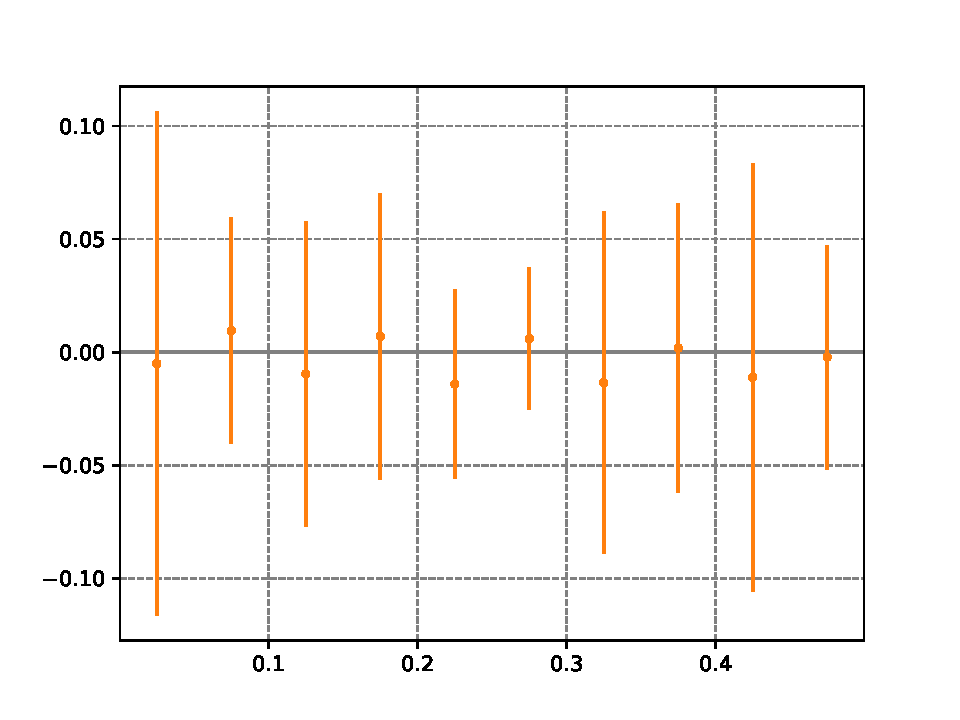
\includegraphics[scale=0.40]{grafico_residui.pdf}
	\caption{Grafico dei residui}
\end{wrapfloat} 
\par\noindent\smallskip Osservando i grafici dei residui, si osserva che sono presenti molti punti che sono negativi: ciò vorrebbe dire che abbiamo misurato dei valori che sono inferiori al nostro modello teorico. Questo potrebbe essere spiegato dal fatto che è sempre presente un errore sistematico, dovuto al nostro apparato sperimentale, dovuto all'attrito dell'aria e del perno di oscillazione: durante le misurazioni noi, infatti, contavamo un'oscillazione quando il pendolo raggiungeva l'oscillazione massima, tuttavia i vari attriti agenti nel sistema hanno rallentato nel tempo la velocità del pendolo, diminuendone conseguentemente le ampiezze e portandoci quindi a misurare dei periodi di oscillazioni minori. I residui invece positivi, secondo la nostra ipotesi, sarebbero allora quelli in cui ha influito maggiormente l'errore dovuto ai nostri tempi di reazione, piuttosto che agli attriti, portandoci quindi a misurare dei periodi di oscillazione maggiori a quelli previsti dal nostro modello teorico.
\newpage

% L'idea migliore sarebbe quello di suddividere in pezzi il codice e di commentarne il funzionamento. Valutare con gli altri
\begin{wrapfloat}{figure}{r}{12cm}
	\begin{lstlisting}[language=Python]
import numpy as np
import math
from matplotlib import pyplot as plt 
from scipy.optimize import curve_fit
data = np.loadtxt(fname="dati.txt", dtype=np.float64)
class Number:
    def __init__(self, arr):
        self.x = arr
        self.n = 7
        self.average_value = 0
    def media(self):
        sum = 0
        for x in self.x:
            sum = sum + x
        self.average_value = sum/len(self.x)
        return(self.average_value)
    def deviazione_standard(self):
        sum = 0
        if self.average_value != 0:
            for x in self.x:
                sum = sum + pow(x - self.average_value, 2)
        self.deviazione = math.sqrt(sum * (len(self.x)))
        return(self.deviazione)
T = np.ones(len(data))
sigma_T = np.ones(len(data))
for el in range(0, len(data)):
    arr = Number(data[el])
    T[el] = arr.media()
    sigma_T[el] = arr.deviazione_standard()
T = T/10
sigma_T = sigma_T/10
L = np.array([0.95, 0.85, 0.75, 0.65, 0.55, 0.45, 0.35, 0.25, 0.15, 0.05])
d = abs(L - 0.525)
sigma_d = np.full(d.shape, 0.002) 
g = 9.81 
def period_model(d, l): 
    """Modello per il periodo del pendolo. 
    """ 
    return 2.0 * np.pi * np.sqrt((l**2.0 / 12.0 + d**2.0) / (g * d)) 
plt.figure("Periodo")
# Scatter plot dei dati. 
plt.errorbar(d, T, sigma_T, sigma_d, fmt="o")  
popt, pcov = curve_fit(period_model, d, T, sigma=sigma_T) 
l_hat = popt[0] 
sigma_l = np.sqrt(pcov[0, 0]) 
print(l_hat, sigma_l) 
x = np.linspace(0.01, 0.5, 100) 
plt.plot(x, period_model(x, l_hat))
plt.errorbar(d, T, yerr=sigma_T, xerr=sigma_d, fmt='.') 
plt.xlabel("d [m]") 
plt.ylabel("Periodo [s]")
plt.grid(which="both", ls="dashed", color="gray")
r = T - period_model(d, l=1.05)
sigma_r = sigma_T
plt.savefig("massa_raggio.pdf") 
plt.show()
plt.plot(d, r, linestyle='', marker='.')
plt.axhline(y = 0, color = 'gray', linestyle = '-') 
plt.errorbar(d, r, sigma_r, sigma_d, fmt=".")
plt.show()
	\end{lstlisting}
\end{wrapfloat}
\end{document}
